\documentclass[12pt,preprint]{aastex}
\usepackage{geometry,amsmath}
\usepackage{float}
%\usepackage{titlesec} %used to format titles
\usepackage{graphicx} %for handling figures
%\usepackage[none]{hyphenat} %disallows hyphenated words


\begin{document}

\title{HERA Dish Reflectometry} 
\author{Zaki Ali, Carina Cheng, Aaron Parsons, Nipanjana Patra}
\maketitle

\section{Introduction}

There are several different sources of instrumental chromaticity for an interferometer such as HERA that each introduce unwanted systematics in data. One such source results from the antenna, which can introduce non-spectrally smooth structure in data due to delays associated with internal signal reflections. The HERA element was designed to minimize this structure - the contamination outside the foreground `wedge' - so that the expected level of the 21cm reionization signal that we are interested in still dominates this region. In order to achieve this, a chromaticity specification of -60dB at 60ns was implemented in the HERA element design, setting a constraint on the level of reflections. In other words, when a signal that originates at the feed re-enters the feed after a time delay of 60ns, it must be attenuated by at least 60dB. 

Understanding the nature of antenna reflections in the HERA dish is of the utmost importance in characterizing the performance of the dish. As HERA progresses as an experiment, it is necessary to build optimal dishes that promise to minimize the challenges of chromaticity in our quest for the Epoch of Reioinization.

\section{Theory}{\label{sec:theory}}

*what is the measurement we are actually doing. 

*compare cable pulse measurements vs. actual sky measurements and how the amount of signal that is transmitted/reflected is different*

*explain why the level of the measurements has to be brought down, and how this is okay for high delays*

\begin{figure}
\centering
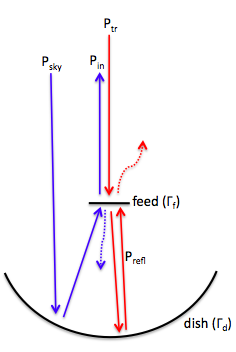
\includegraphics[totalheight=0.5\textheight]{plots/reflection_cartoon.png}
\caption{The blue solid lines represent an original sky signal entering the feed. A small percentage of it (dashed blue) is reflected off the dish, and it is these reflections that we are concerned about. In our measurements however, the reflections measured contain most of the original pulse signal (solid red), so it is crucial to adjust for this difference in our analysis.}
\end{figure}

\section{Methodology}

To measure the delays associated with reflections within the dish and feed, we
used the prototype HERA dish (Figure \ref{fig:heradish} built at the NRAO site in
Green Bank, WV. The dish is a 14-m parabolic reflector structurally supported
with 3 telephone poles. The reflective material is made up of wire mesh that
is attached to PVC pipes that form the parabolic shape. With the current
prototype, the feed is a PAPER dipole encased in a cylindrical cage encompassing
the backplane. The PAPER feed and the backplane (which prevents feed-to-feed
interaction between neighboring dishes) is raised and lowered by a three-pulley
system. The focal height of the dish is 4.5m ($\sim{14.76}$ft). Feed heights quoted in our measurements represent the distance from the balun to the top of the central concrete hub. Note, however, that the actual focal height of the dish represents the distance from the backplane of the feed to the dish's wire mesh, which intersects the concrete hub between the ground and the top of the hub. 
%XXX get discrepancy distance from DaveD.

The following reflectometry measurements were taken on July 20-23, 2015 using a
FieldFox unit in Network Analyzer mode. A pulse is generated in the FieldFox
and sent through a 75ft $50\Omega$ cable that connects to the feed with a 4:1
passive balun. The return loss as a function of frequency is saved. Both
the amplitude of the power and phase information are saved. Our
measurements are taken for a frequency bandwidth of 50 to 500MHz. 

Measurements are transformed into the delay domain during post-processing so that window functions
can be used in the Fourier transform. Without a window function, taking the Fourier transform of a finite data series (such as the return loss over a finite bandwidth), which can be interpreted as a square window function, is equivalent to convolving the Fourier transformed data with a $sinc$ function. This results in excess power at high delays due to the sidelobes in the $sinc$ function. Consequently, we have chosen to use a Blackman-Harris window function when moving into the delay domain. The effectiveness of this window function compared to a square window function is illustrated in Figure \ref{fig:window}.

\begin{figure}
\centering
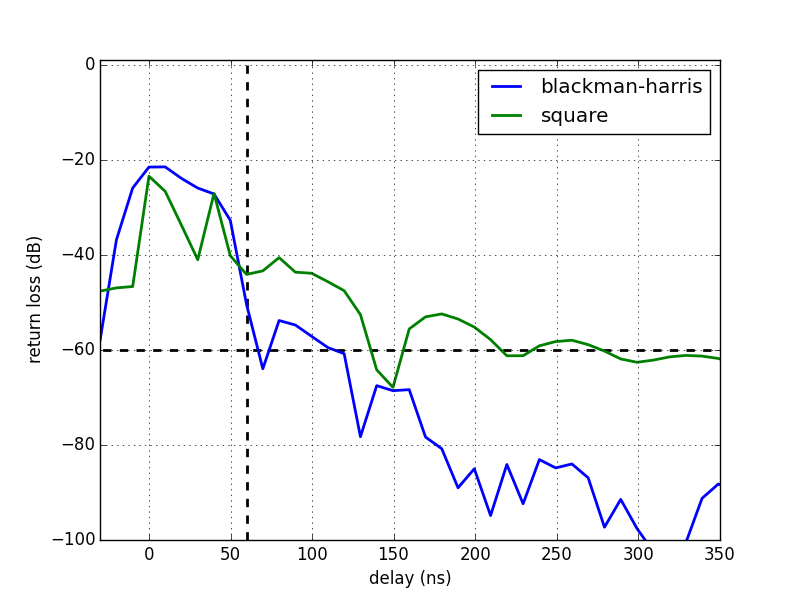
\includegraphics[totalheight=0.5\textheight]{plots/bh_vs_sq.png}
\caption{Delay plot produced using a Blackman-Harris window function vs. a square window function for the PAPER bandwidth.}
\label{fig:window}
\end{figure}

As mentioned in Section \ref{sec:theory}, there is a mis-match in amplitude between the reflections that we measure (originating from the FieldFox pulse) and reflections produced by sky signal. To compensate, we multiply our entire windowed delay spectrum by the DC component of the un-windowed delay spectrum.

\begin{figure}
\centering
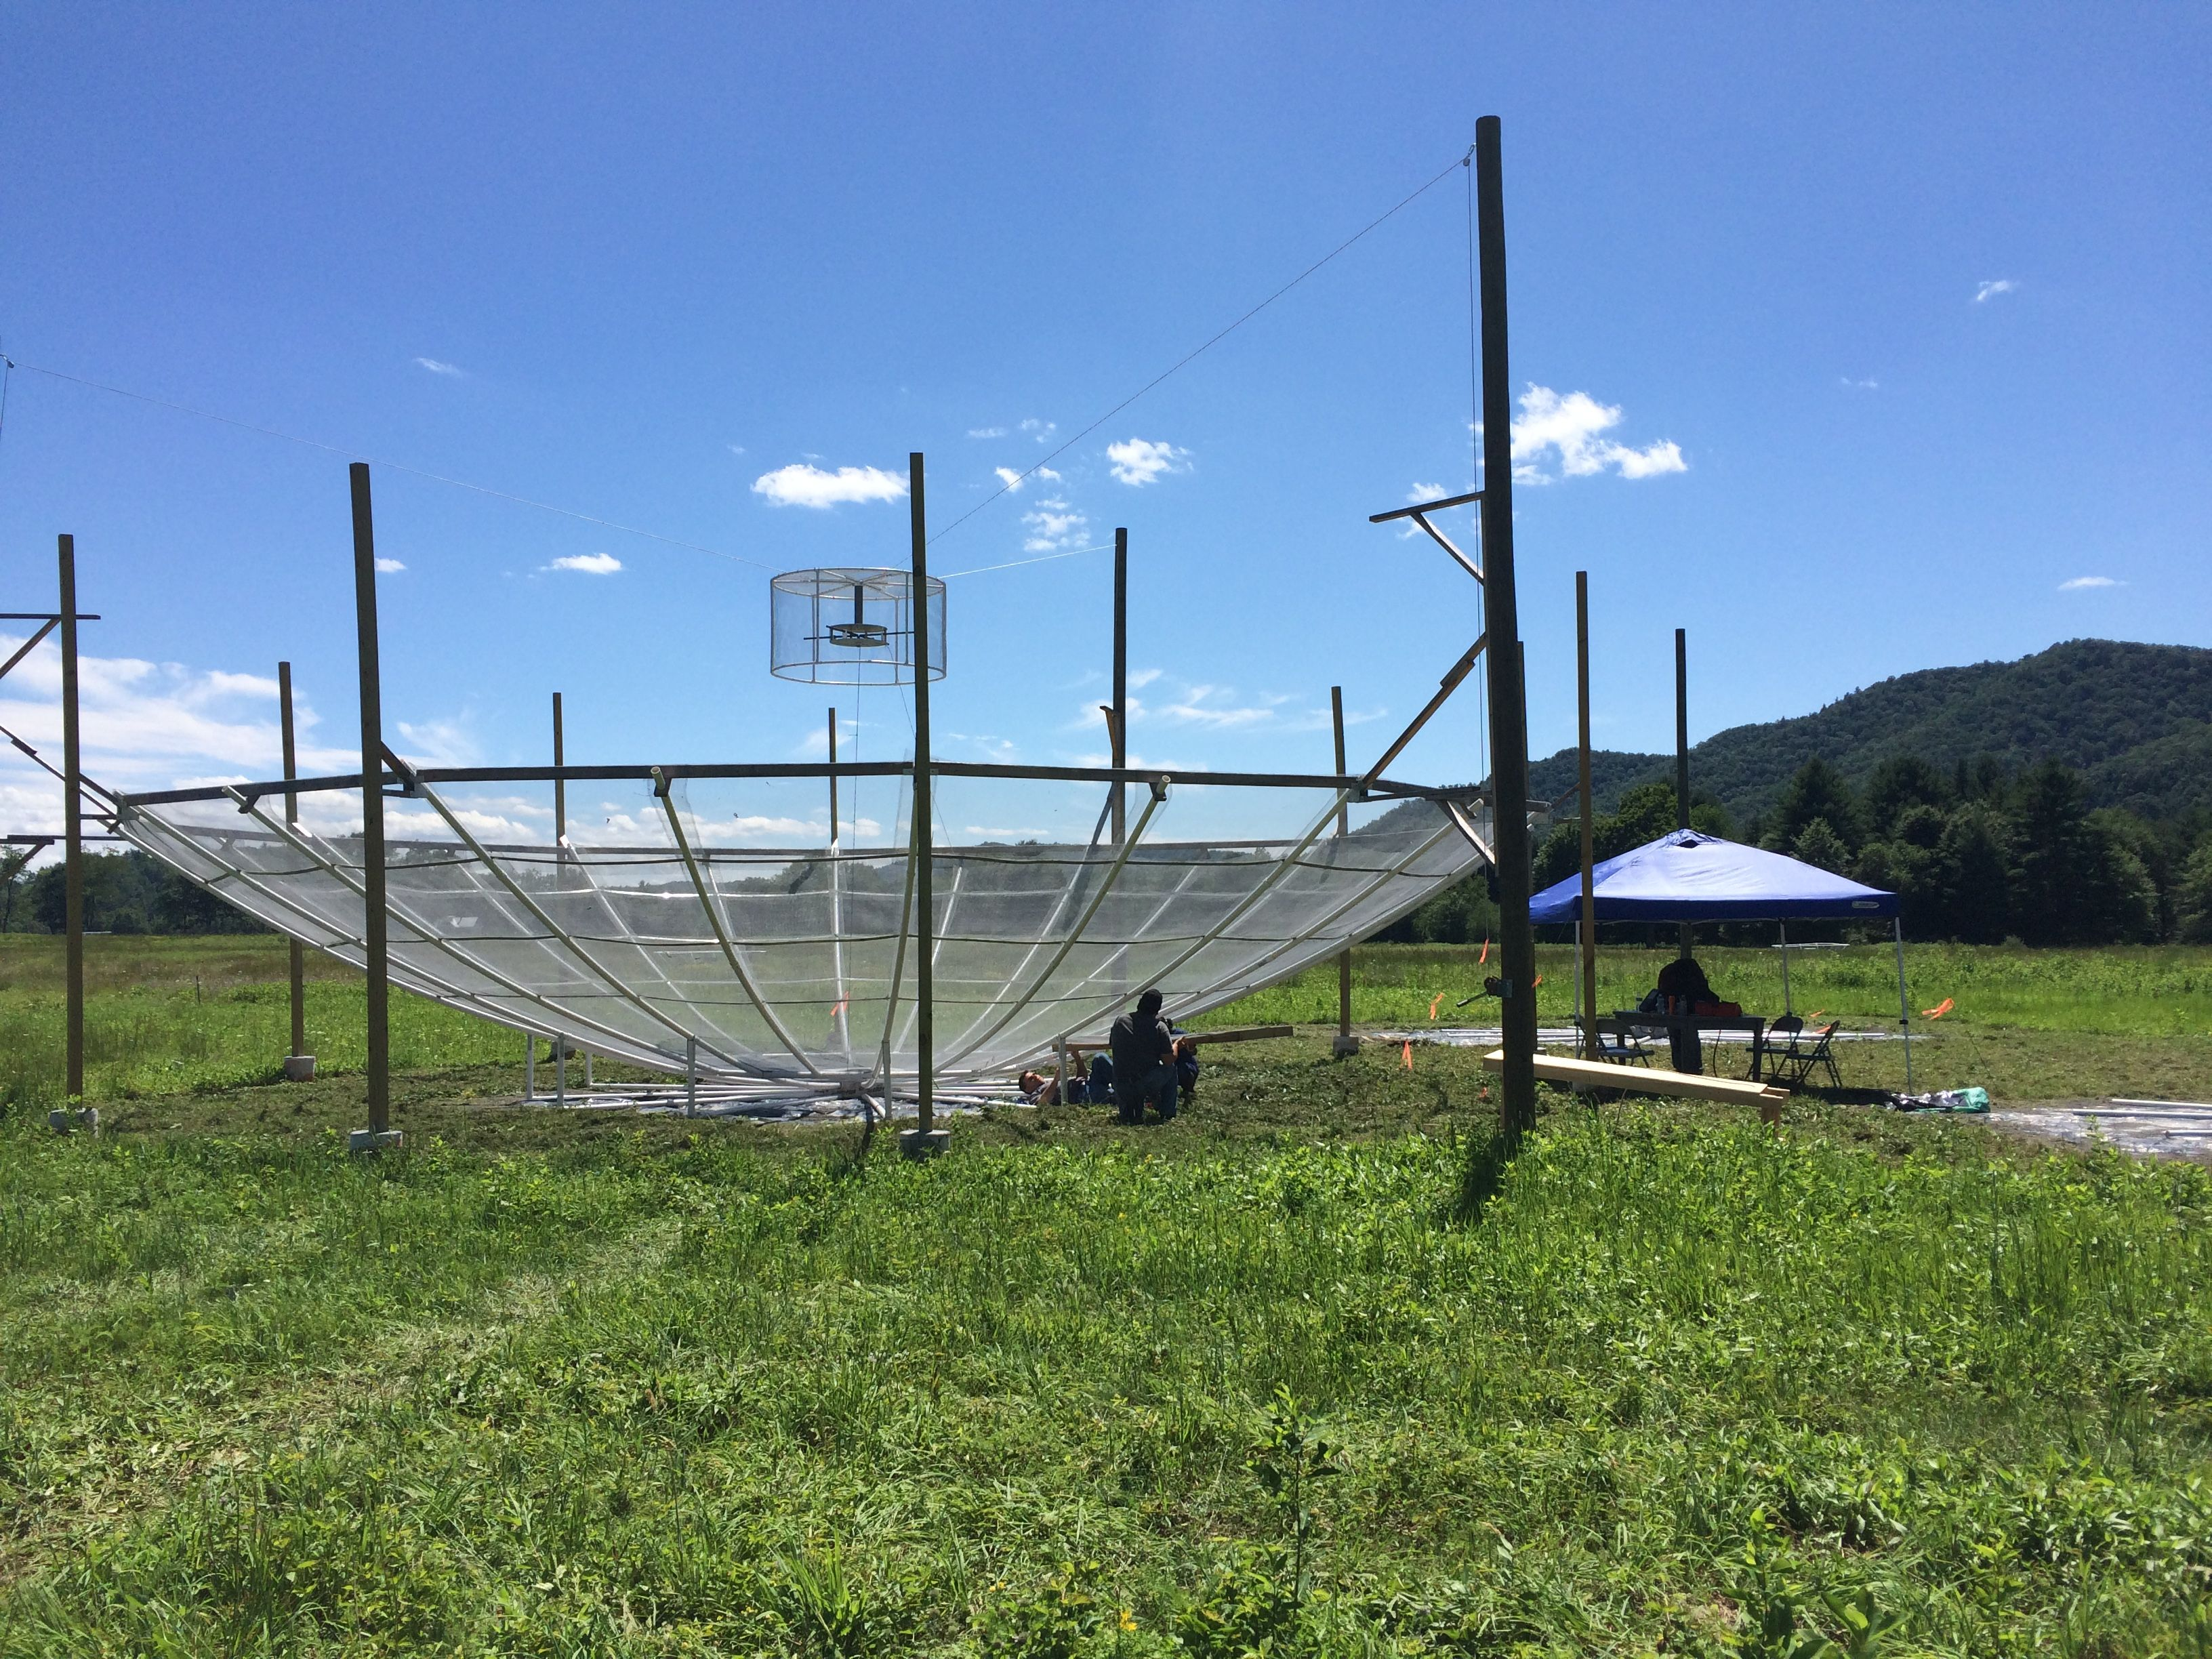
\includegraphics[trim={2cm 20cm 30cm 15cm},clip, totalheight=0.45\textheight]{plots/heradish.jpg}
\caption{HERA dish and feed at the Green Bank NRAO site.}
\label{fig:heradish}
\end{figure}

\section{Results}

Figure \ref{fig:freq} shows the return loss for a frequency bandwidth of 50 to 500MHz. This measurement was taken with the feed suspended at 12ft (distance between the balun and top of the central concrete hub). Because the return loss is the ratio of the power received to the power transmitted, higher reflections can clearly be seen outside of the PAPER bandwidth. This is not surprising, since the feed is tuned specifically for PAPER. The return loss minima are locations where our feed is well-matched to free space.

\begin{figure}
\centering
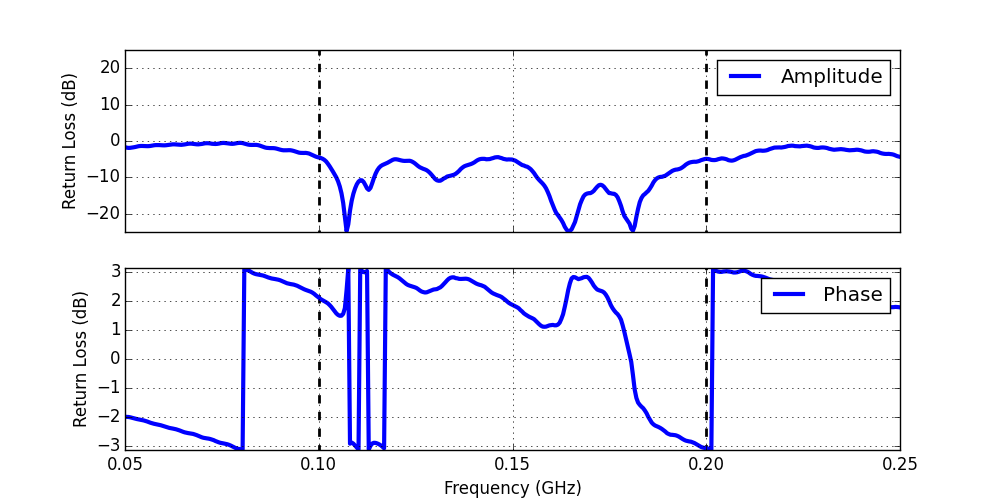
\includegraphics[totalheight=0.4\textheight]{plots/frequency_amp_phase.png}
\caption{Amplitude and phase of the measured return loss.}
\label{fig:freq}
\end{figure}

In Figure \ref{fig:3bands}, the return loss is plotted versus delay for three chosen bandwidths: the HERA bandwidth, the PAPER bandwidth, and a typical power spectra bandwidth when using a Blackman-Harris window function. It is again shown that the reflections are minimized for the PAPER bandwidth. 

\begin{figure}
\centering
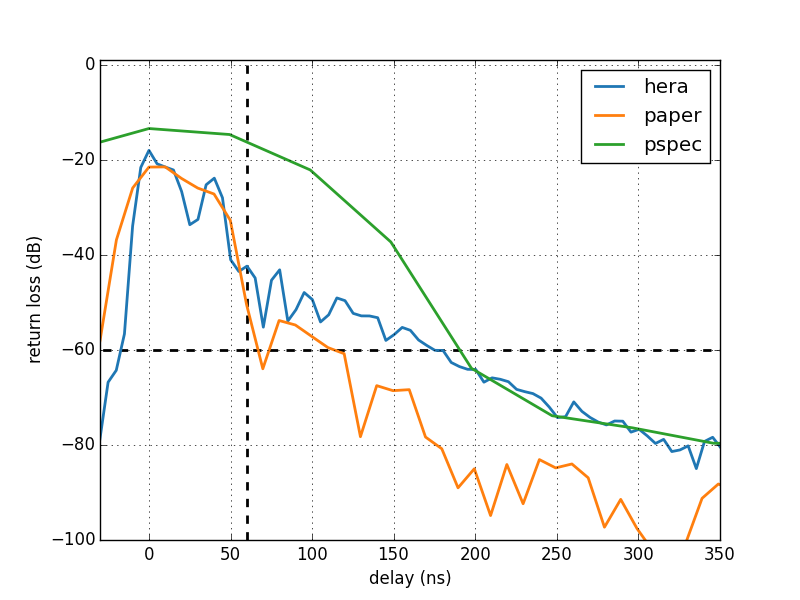
\includegraphics[totalheight=0.5\textheight]{plots/delay3_window.png}
\caption{Delay plots produced using a Blackman-Harris window function for 3 different frequency bandwidths: 50MHz-250MHz (``hera"), 100MHz-200MHz (``paper"), and 140MHz-160MHz (``pspec"). The black dashed lines illustrate our ``60 by 60" specification.}
\label{fig:3bands}
\end{figure}

Figure \ref{fig:elevator} is again a delay plot of the return loss, but for four different feed suspension heights. We use the PAPER bandwidth and note that the measurements are near identical at low delays, implying that low delay reflections are caused primarily by reflections within the feed cage. However, at higher delays we notice discrepancies between the different heights.

\begin{figure}
\centering
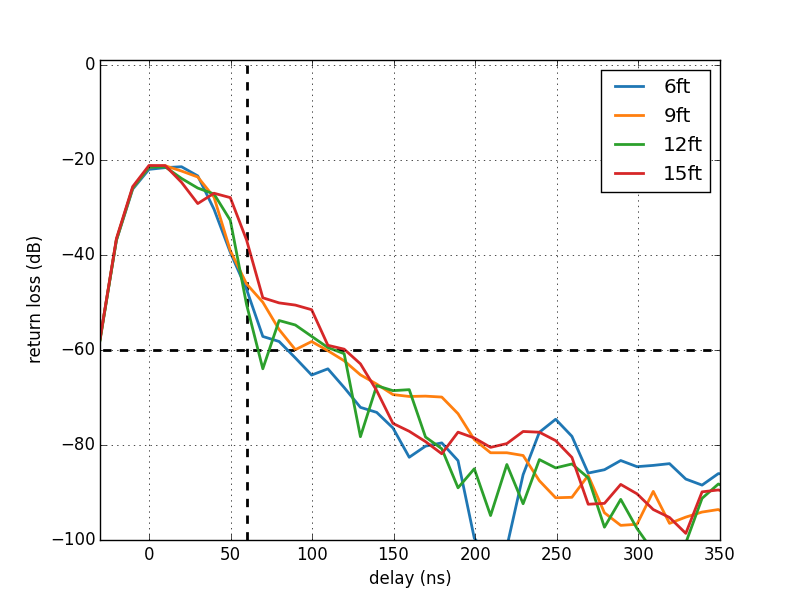
\includegraphics[totalheight=0.5\textheight]{plots/delay_heights_paper.png}
\caption{Delay plots produced using a Blackman-Harris window function for 4 different feed heights and the PAPER bandwidth. The black dashed lines illustrate our ``60 by 60" specification.}
\label{fig:elevator}
\end{figure}

Finally, Figure \ref{fig:outofthedish} presents measurements taken of the feed away from the dish. Echosorb is placed under the feed for some of the measurements, with the expectation that it will prevent any reflections off the ground. Measurements are also taken of the feed inside its metal cage in various configurations. 

\begin{figure}
\centering
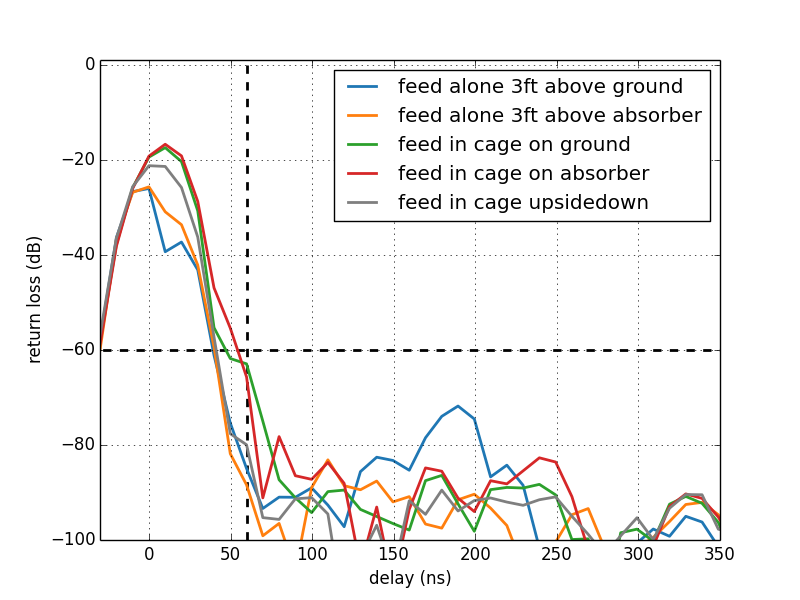
\includegraphics[totalheight=0.5\textheight]{plots/delay_feed.png}
\caption{Delay plots produced using a Blackman-Harris window function for different lone feed configurations and the PAPER bandwidth. The black dashed lines illustrate our ``60 by 60" specification.}
\label{fig:outofthedish}
\end{figure}


\section{Conclusion}


\end{document}
